%%%%%%%%%%%%%%%%%%%%%%%%%%%%%%%%%%%%%%%%%
% Beamer Presentation
% LaTeX Template
% Version 1.0 (10/11/12)
%
% This template has been downloaded from:
% http://www.LaTeXTemplates.com
%
% License:
% CC BY-NC-SA 3.0 (http://creativecommons.org/licenses/by-nc-sa/3.0/)
%
%%%%%%%%%%%%%%%%%%%%%%%%%%%%%%%%%%%%%%%%%

%----------------------------------------------------------------------------------------
%	PACKAGES AND THEMES
%----------------------------------------------------------------------------------------

%\documentclass[UTF8,aspectratio=169,14pt]{ctexbeamer}
\documentclass[UTF8,aspectratio=169]{ctexbeamer}
\usepackage{hyperref}
\hypersetup{
	colorlinks=true,
	linkcolor=red,
	anchorcolor=blue,
	citecolor=green
}

\mode<presentation> {
	
	% The Beamer class comes with a number of default slide themes
	% which change the colors and layouts of slides. Below this is a list
	% of all the themes, uncomment each in turn to see what they look like.
	
	%\usetheme{default}
	%\usetheme{AnnArbor}
	%\usetheme{Antibes}
	%\usetheme{Bergen}
	%\usetheme{Berkeley}
	%\usetheme{Berlin}
	%\usetheme{Boadilla}
	%\usetheme{CambridgeUS}
	%\usetheme{Copenhagen}
	%\usetheme{Darmstadt}
	%\usetheme{Dresden}
	%\usetheme{Frankfurt}
	%\usetheme{Goettingen}
	%\usetheme{Hannover}
	%\usetheme{Ilmenau}
	%\usetheme{JuanLesPins}
	%\usetheme{Luebeck}
	\usetheme{Madrid}
	%\usetheme{Malmoe}
	%\usetheme{Marburg}
	%\usetheme{Montpellier}
	%\usetheme{PaloAlto}
	%\usetheme{Pittsburgh}
	%\usetheme{Rochester}
	%\usetheme{Singapore}
	%\usetheme{Szeged}
	%\usetheme{Warsaw}
	
	% As well as themes, the Beamer class has a number of color themes
	% for any slide theme. Uncomment each of these in turn to see how it
	% changes the colors of your current slide theme.
	
	%\usecolortheme{albatross}
	%\usecolortheme{beaver}
	%\usecolortheme{beetle}
	%\usecolortheme{crane}
	%\usecolortheme{dolphin}
	%\usecolortheme{dove}
	%\usecolortheme{fly}
	%\usecolortheme{lily}
	%\usecolortheme{orchid}
	%\usecolortheme{rose}
	%\usecolortheme{seagull}
	%\usecolortheme{seahorse}
	%\usecolortheme{whale}
	%\usecolortheme{wolverine}
	
	%\setbeamertemplate{footline} % To remove the footer line in all slides uncomment this line
	%\setbeamertemplate{footline}[page number] % To replace the footer line in all slides with a simple slide count uncomment this line
	
	%\setbeamertemplate{navigation symbols}{} % To remove the navigation symbols from the bottom of all slides uncomment this line
}

\usepackage{graphicx} % Allows including images
\graphicspath{{./figs/}}
\usepackage{booktabs} % Allows the use of \toprule, \midrule and \bottomrule in tables
\usepackage{longtable}
\usepackage{listings}
\usepackage{xcolor}
\lstset{numbers=left, %设置行号位置
	numberstyle=\tiny, %设置行号大小
	keywordstyle=\color{blue}, %设置关键字颜色
	commentstyle=\color[cmyk]{1,0,1,0}, %设置注释颜色
	frame=single, %设置边框格式
	escapeinside=``, %逃逸字符(1左面的键),用于显示中文
	%breaklines, %自动折行
	extendedchars=false, %解决代码跨页时,章节标题,页眉等汉字不显示的问题
	xleftmargin=2em,xrightmargin=2em, aboveskip=1em, %设置边距
	tabsize=4, %设置tab空格数
	showspaces=false %不显示空格
}
% Fonts
% \usepackage{libertine}
% \setmonofont{Courier}
\setCJKsansfont[ItalicFont=Noto Serif CJK SC Black, BoldFont=Noto Sans CJK SC Black]{Noto Sans CJK SC}
\setmainfont[Ligatures={Common,TeX}]{Linux  Libertine O}
\setmonofont[SmallCapsFont={Latin Modern Mono Caps}]{Latin Modern Mono Light}
\setsansfont{Linux Biolinum O}

\logo{
\includegraphics[width=0.55cm,height=0.55cm]{../../thcs-logo.png}}

%----------------------------------------------------------------------------------------
%	TITLE PAGE
%----------------------------------------------------------------------------------------

\title[第14讲]{第14讲: Concurrency in OS Kernel} % The short title appears at the bottom of every slide, the full title is only on the title page
\subtitle{第二节:Scalable Concurrency -- Lock}
\author{陈渝} % Your name
\institute[清华大学] % Your institution as it will appear on the bottom of every slide, may be shorthand to save space
{
	清华大学计算机系 \\ % Your institution for the title page
	\medskip
	\textit{yuchen@tsinghua.edu.cn} % Your email address
}
\date{\today} % Date, can be changed to a custom dateC++ memory order



\begin{document}

\begin{frame}
\titlepage % Print the title page as the first slide
\end{frame}
    
%\begin{frame}
%\frametitle{提纲} % Table of contents slide, comment this block out to remove it
%\tableofcontents % Throughout your presentation, if you choose to use \section{} and \subsection{} commands, these will automatically be printed on this slide as an overview of your presentation
%\end{frame}
%
%%----------------------------------------------------------------------------------------
%%	PRESENTATION SLIDES
%%----------------------------------------------------------------------------------------
%

%----------------------------------------------
%-------------------------------------------------
\begin{frame}
    \frametitle{Resource}
    
    
    

	\begin{columns}
    
    \begin{column}{.5\textwidth}
        \centering
        
        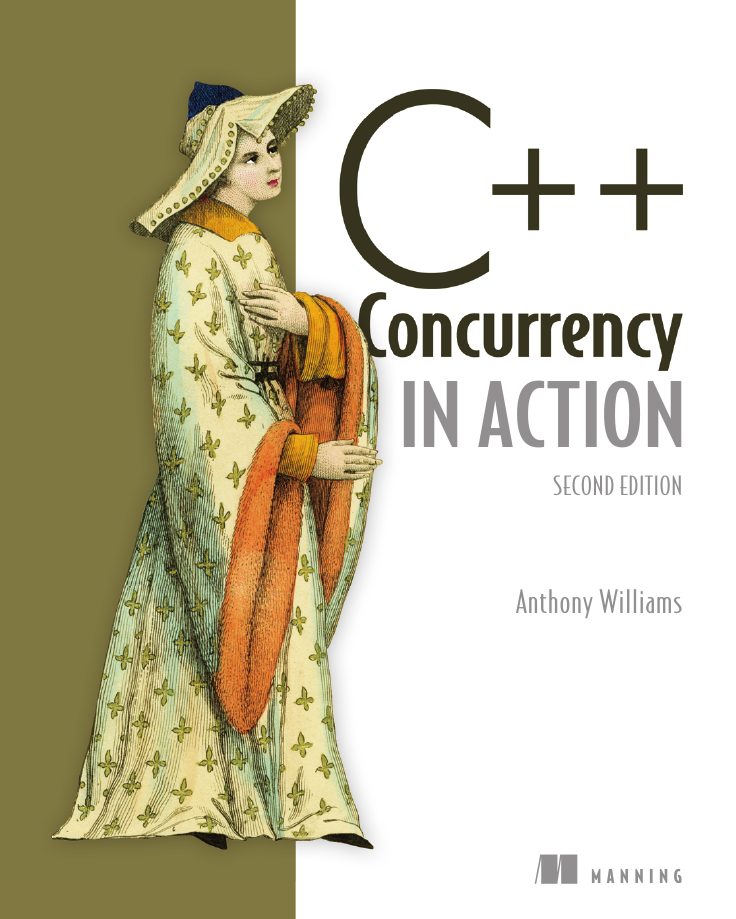
\includegraphics[width=.7\textwidth]{book-cpp-concurrency-in-action}
        
    \end{column}
    
    \begin{column}{.5\textwidth}
        
      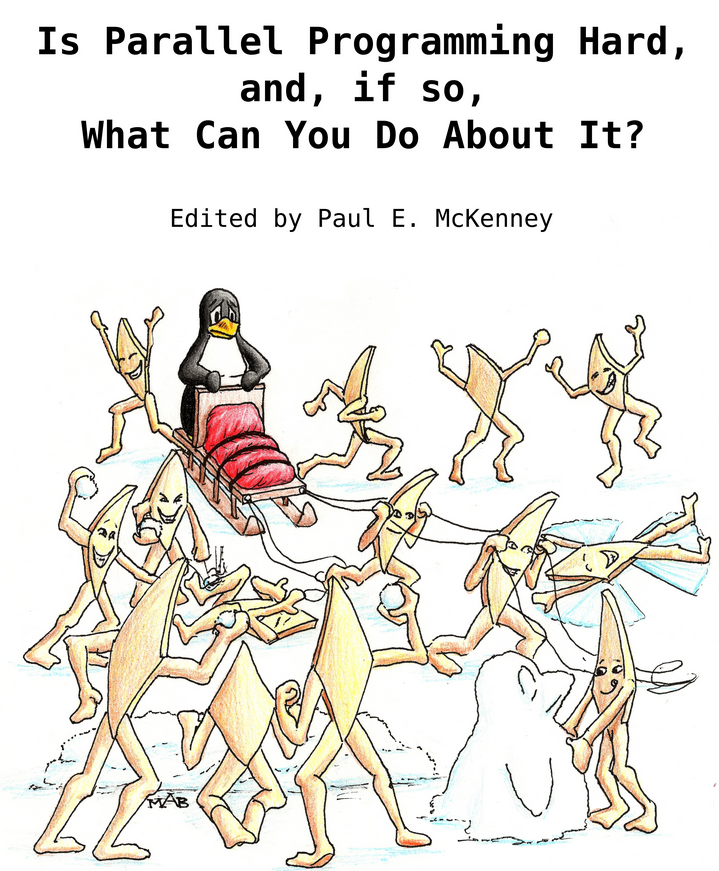
\includegraphics[width=.7\textwidth]{perfbook}
       
        
    \end{column}
    
    
\end{columns}
    
    \tiny Reference:
    
    "Is Parallel Programming Hard, And, If So, What Can You Do About It?",Paul McKenney;\\
    "C++Concurrency in Action", ANTHONY WILLIAMS; \\
    "CS510 - Advanced Topics in Concurrency", Jonathan Walpole;
    Adam Belay from MIT PDOS
\end{frame}

%----------------------------------------------
\begin{frame}[fragile]
    \frametitle{Scalable Locking}
    \Large
    \begin{itemize}
    \item Why do we need locking in the kernel?
    \item Which problems are we trying to solve?
    \item What implementation choices do we have?
    \item Is there a one-size-fits-all solution?
  
\end{itemize}
    
\end{frame}


%----------------------------------------------
\begin{frame}[fragile]
    \frametitle{ticket spinlock}
    \Large
    Goal
    \begin{itemize}
        \item Correctness:  Mutual exclusion, Progress, Bounded wait
        \item  Fairness       
        \item Performance
        
        
    \end{itemize}
    
\end{frame}


%----------------------------------------------
\begin{frame}[fragile]
    \frametitle{ticket spinlock}
    \Large
    Idea:
    \begin{itemize}
        \item reserve each thread's turn to use a lock
        \item each thread spins until their turn
        \item Use new atomic primitive:
        fetch-and-add (FAA)
        \item Spin while not thread's ticket != turn
        \item Release: Advance to next turn
        
 \end{itemize}
    
\end{frame}


%----------------------------------------------
\begin{frame}[fragile]
    \frametitle{ticket spinlock}
%    \large    
    \begin{block}{}
        \begin{verbatim}
typedef  struct {
    int ticket;
    int turn;
} lock_t;

void lock_init(lock_t *lock) {
    lock->ticket = 0;
    lock->turn = 0;
}
void acquire(lock_t *lock) {
    int myturn = FAA(&lock->ticket);
    while (lock->turn != myturn); // spin
}
void release(lock_t *lock) { lock->turn += 1; }

        \end{verbatim}
    \end{block} 
\end{frame}

%----------------------------------------------
\begin{frame}[fragile]
    \frametitle{ticket spinlock}
    \Large
    Ticket lock time analysis
    
    \begin{itemize}
        \item Atomic increment – O(1) broadcast message        
        \item Then read-only spin, no cost until next release             
        \item  release OP invalidates message sent to all cores, and O(N) find messages, as they re-read        
        \item  But fairness and less bus traffic while spinning
        
        
    \end{itemize}
    Ticket are “non-scalable” locks, cost of handoff scales with number of waiters
    
    
\end{frame}
%----------------------------------------------
\begin{frame}[fragile]
    \frametitle{MCS lock}
    \Large

    \begin{itemize}
        \item Goal: O(1) message release time
        \item Can we wake just one core at a time?
        \item  Idea: Have each core spin on a different cache-line
    \end{itemize}    
\end{frame}

%----------------------------------------------
\begin{frame}[fragile]
    \frametitle{MCS lock}
    \Large
    
    \begin{itemize}
        \item Each CPU has a qnode structure in its local memory

    \begin{block}{}
    \begin{verbatim}
    typedef struct qnode {
        struct qnode *next;
        bool locked;
    } qnode;
\end{verbatim}
\end{block}         
        \item  A lock is a qnode pointer to the tail of the list      
        \item While waiting, spin on local locked flag
        
    \end{itemize}    
\end{frame}

%----------------------------------------------
\begin{frame}[fragile]
    \frametitle{MCS lock}
\centering
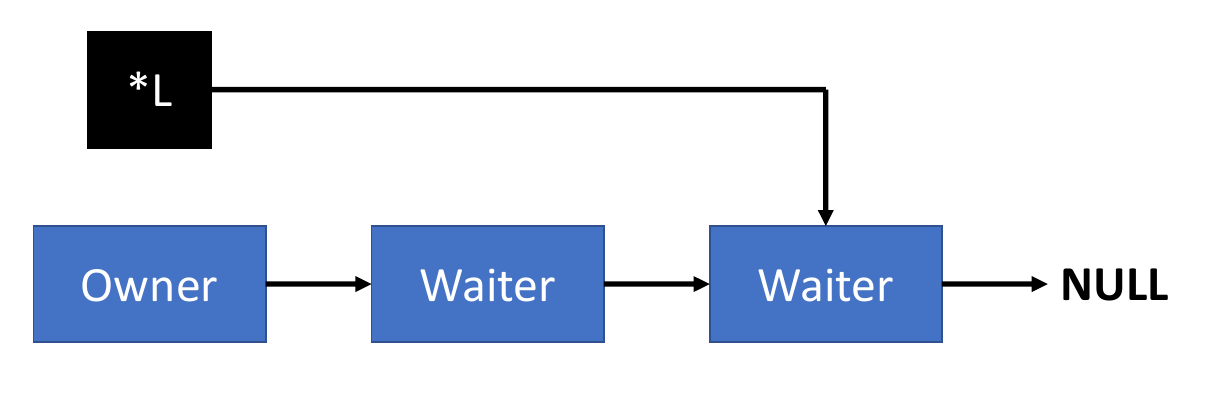
\includegraphics[width=1.\textwidth]{mcs-lock}
\end{frame}



%----------------------------------------------
\begin{frame}[fragile]
    \frametitle{MCS lock}
    \Large
     Acquiring MCS locks
       
        \begin{block}{}
            \begin{verbatim}
acquire (qnode *L, qnode *I) {
    I->next = NULL;
    qnode *predecessor = I;
    XCHG (*L, predecessor);
    if (predecessor != NULL) {
        I->locked = true;
        predecessor->next = I;
        while (I->locked) ;
    }
}
\end{verbatim}
        \end{block}         

\end{frame}


%----------------------------------------------
\begin{frame}[fragile]
    \frametitle{MCS lock}
    \Large
    Releasing MCS locks
    
    \begin{block}{}
        \begin{verbatim}
    release (lock *L, qnode *I) {
        if (!I->next)
            if (CAS (*L, I, NULL))
                return;
        while (!I->next) ;
        I->next->locked = false;
    }
\end{verbatim}
    \end{block}         
    
\end{frame}



%----------------------------------------------
\begin{frame}[fragile]
    \frametitle{MCS lock}
    \centering
    But not a  panacea
    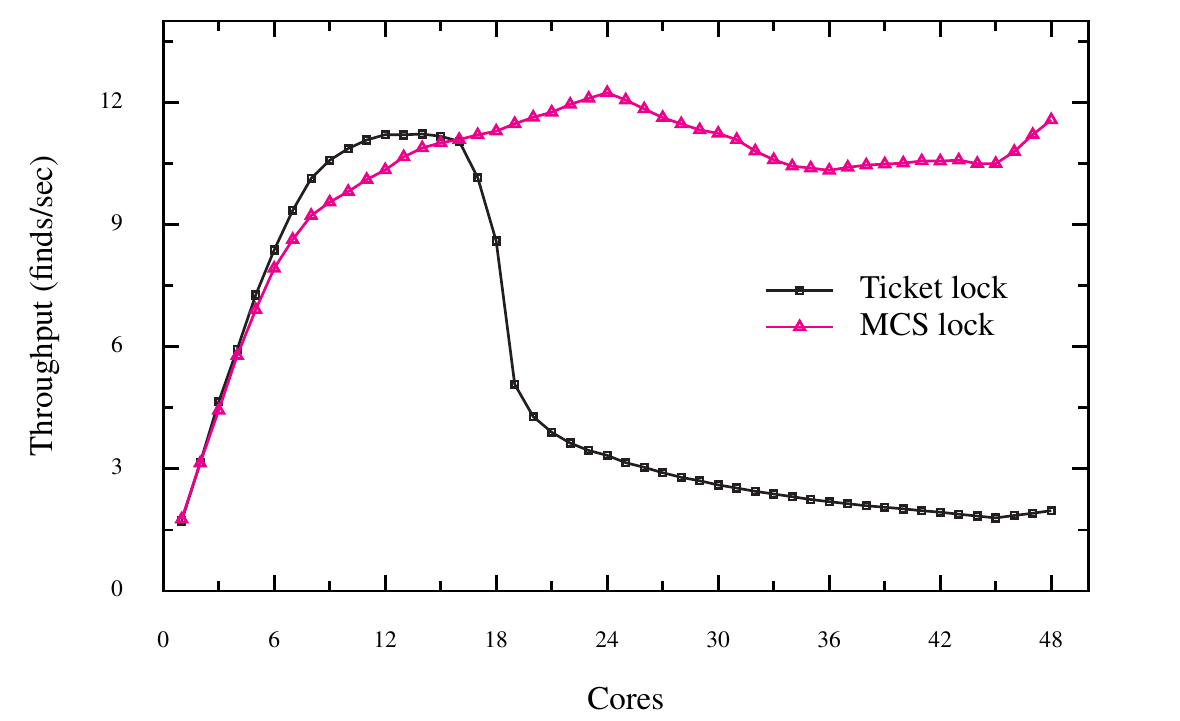
\includegraphics[width=.7\textwidth]{mcs-lock-perf2}
\end{frame}


%----------------------------------------------
\begin{frame}[fragile]
    \frametitle{CLH lock}
    \centering
    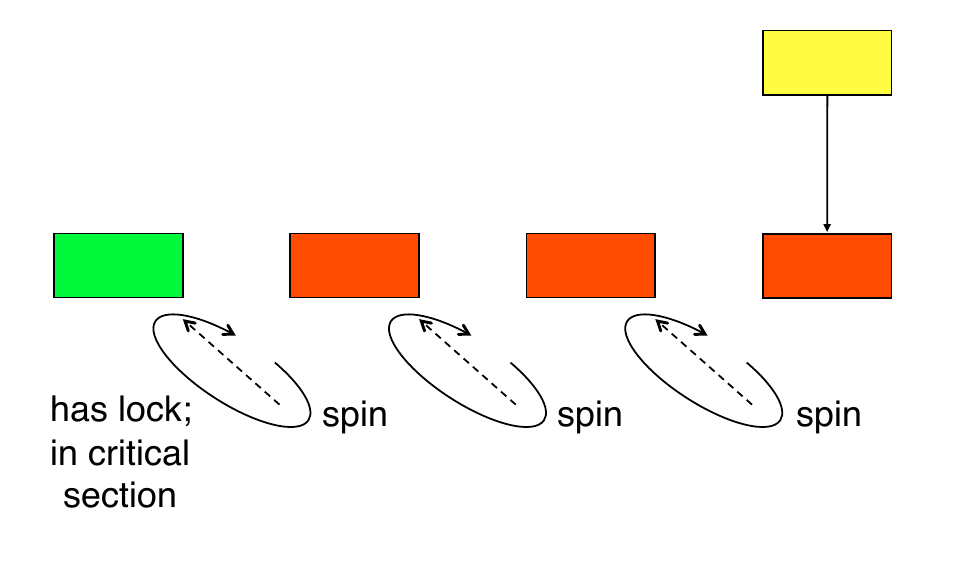
\includegraphics[width=.8\textwidth]{clh-lock}
\end{frame}
%----------------------------------------------
\begin{frame}[fragile]
    \frametitle{CLH lock}    
    \begin{block}{}
        \begin{verbatim}
type qnode = record
    prev : ^qnode
    succ_must_wait : Boolean
    
type lock = ^qnode   // initialized to point to an unowned qnode

procedure acquire_lock (L : ^lock, I : ^qnode)
    I->succ_must_wait := true
    pred : ^qnode := I->prev := fetch_and_store(L, I)
    repeat while pred->succ_must_wait

procedure release_lock (ref I : ^qnode)
    pred : ^qnode := I->prev
    I->succ_must_wait := false
    I := pred    // take pred's qnode
 \end{verbatim}
    \end{block}         
    
\end{frame}

%----------------------------------------------
\begin{frame}[fragile]
    \frametitle{lock comparison}
    \centering
    Locking strategy comparison
    
    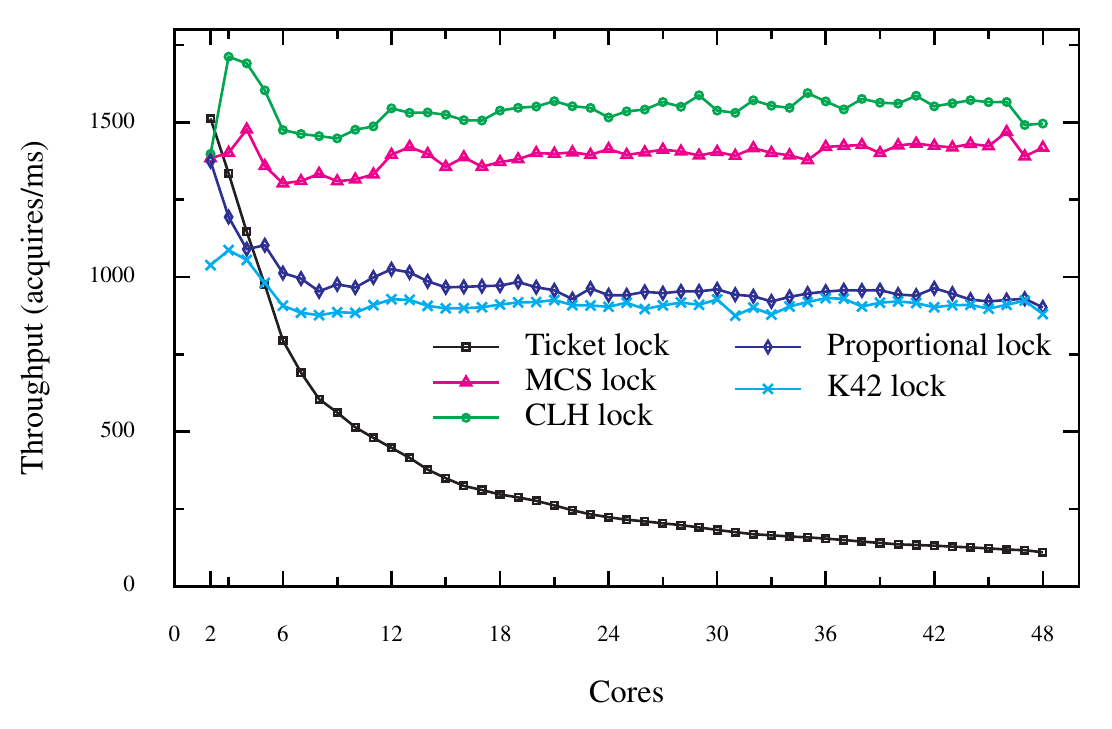
\includegraphics[width=.7\textwidth]{mcs-lock-perf}
\end{frame}


MCS 来自于其发明人名字的首字母: John Mellor-Crummey和Michael Scott。
CLH的发明人是:Craig,Landin and Hagersten。
MCS Spinlock 是一种基于链表的可扩展、高性能、公平的自旋锁,申请线程只在本地变量上自旋,直接前驱负责通知其结束自旋,从而极大地减少了不必要的处理器缓存同步的次数,降低了总线和内存的开销

从代码实现来看,CLH比MCS要简单得多。
从自旋的条件来看,CLH是在前驱节点的属性上自旋,而MCS是在本地属性变量上自旋
从链表队列来看,CLH的队列是隐式的,CLHNode并不实际持有下一个节点;MCS的队列是物理存在的。
CLH锁释放时只需要改变自己的属性,MCS锁释放则需要改变后继节点的属性。

%----------------------------------------------
%----------------------------------------------
\end{document}